\documentclass{standalone}
\usepackage{tikz}
\usetikzlibrary{patterns, positioning}
\usepackage[sfdefault]{ClearSans} %% option 'sfdefault' activates Clear Sans as the default text font
\usepackage[T1]{fontenc}

\begin{document}
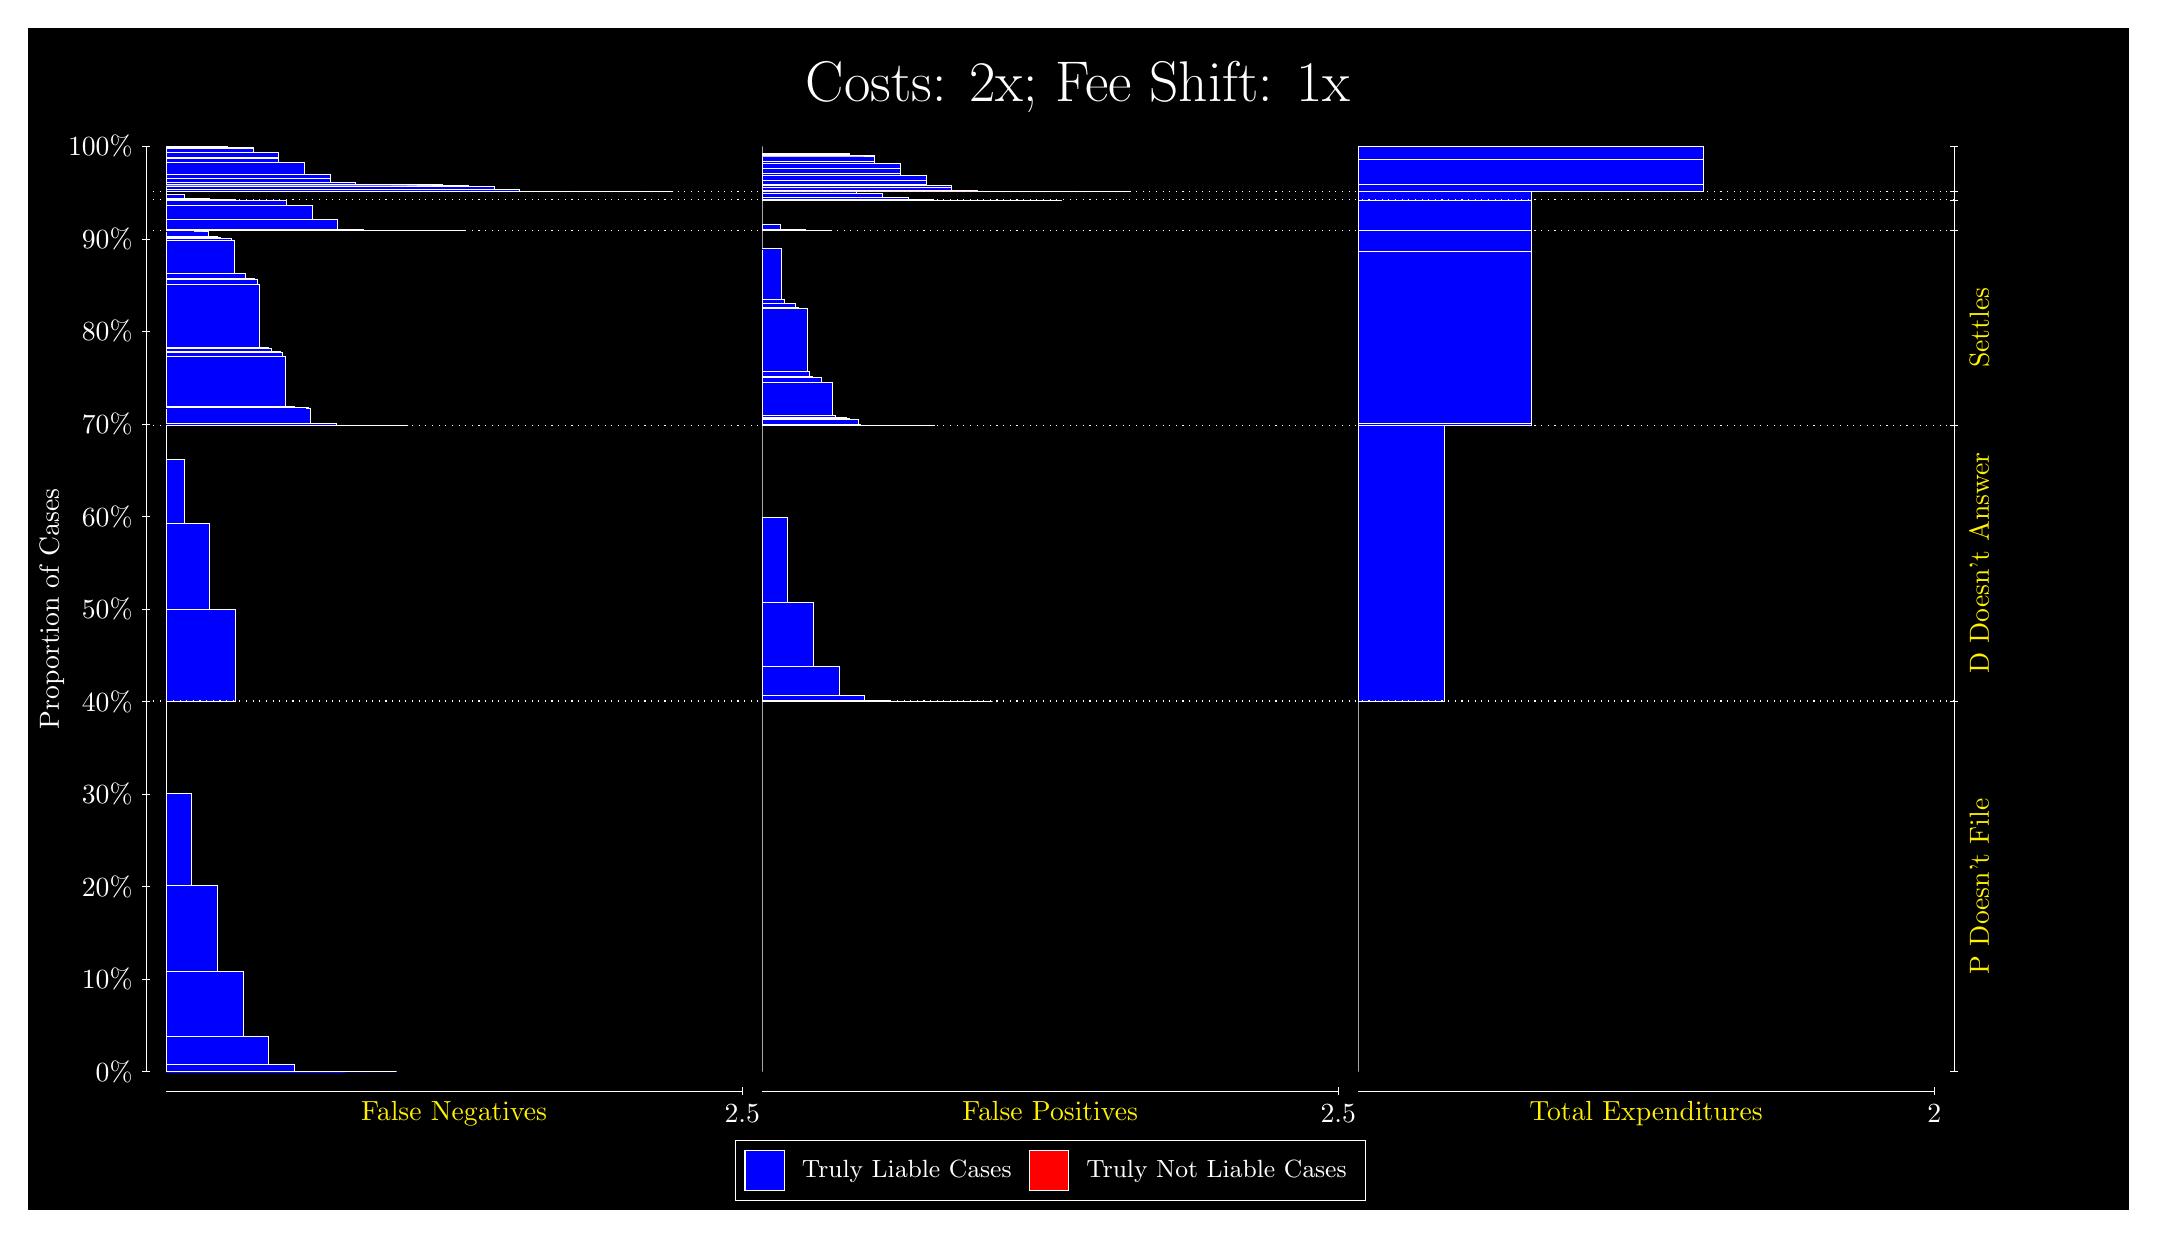
\begin{tikzpicture}
\draw[fill=black] (0,0) rectangle (26.667,15);
\draw[text=white] (0,13.5) rectangle (26.667,15) node[midway] {\huge Costs: 2x; Fee Shift: 1x};
\draw[white, very thin] (1.5,1.75) -- (1.5,13.5);
\node[rotate=90, text=white, anchor=center] at (0.3, 7.625) {Proportion of Cases};
\draw[white, very thin] (1.45,1.75) -- (1.55,1.75);
\node[text=white, anchor=east] at (1.45, 1.75) {0\%};
\draw[white, very thin] (1.45,2.925) -- (1.55,2.925);
\node[text=white, anchor=east] at (1.45, 2.925) {10\%};
\draw[white, very thin] (1.45,4.1) -- (1.55,4.1);
\node[text=white, anchor=east] at (1.45, 4.1) {20\%};
\draw[white, very thin] (1.45,5.275) -- (1.55,5.275);
\node[text=white, anchor=east] at (1.45, 5.275) {30\%};
\draw[white, very thin] (1.45,6.45) -- (1.55,6.45);
\node[text=white, anchor=east] at (1.45, 6.45) {40\%};
\draw[white, very thin] (1.45,7.625) -- (1.55,7.625);
\node[text=white, anchor=east] at (1.45, 7.625) {50\%};
\draw[white, very thin] (1.45,8.8) -- (1.55,8.8);
\node[text=white, anchor=east] at (1.45, 8.8) {60\%};
\draw[white, very thin] (1.45,9.975) -- (1.55,9.975);
\node[text=white, anchor=east] at (1.45, 9.975) {70\%};
\draw[white, very thin] (1.45,11.15) -- (1.55,11.15);
\node[text=white, anchor=east] at (1.45, 11.15) {80\%};
\draw[white, very thin] (1.45,12.325) -- (1.55,12.325);
\node[text=white, anchor=east] at (1.45, 12.325) {90\%};
\draw[white, very thin] (1.45,13.5) -- (1.55,13.5);
\node[text=white, anchor=east] at (1.45, 13.5) {100\%};

\draw[white, very thin] (24.457,1.75) -- (24.457,13.5);
\draw[white, very thin] (24.407,1.75) -- (24.507,1.75);
\node[anchor=west] at (24.407, 1.75) {};
\draw[white, very thin] (24.407,6.4553) -- (24.507,6.4553);
\node[anchor=west] at (24.407, 6.4553) {};
\draw[white, very thin] (24.407,9.9589) -- (24.507,9.9589);
\node[anchor=west] at (24.407, 9.9589) {};
\draw[white, very thin] (24.407,12.433) -- (24.507,12.433);
\node[anchor=west] at (24.407, 12.433) {};
\draw[white, very thin] (24.407,12.819) -- (24.507,12.819);
\node[anchor=west] at (24.407, 12.819) {};
\draw[white, very thin] (24.407,12.93) -- (24.507,12.93);
\node[anchor=west] at (24.407, 12.93) {};
\draw[white, very thin] (24.407,13.5) -- (24.507,13.5);
\node[anchor=west] at (24.407, 13.5) {};

\draw[white, very thin, fill=blue] (1.75,1.75) rectangle (4.6775,1.75);
\draw[white, very thin, fill=blue] (1.75,1.75) rectangle (4.3523,1.75);
\draw[white, very thin, fill=blue] (1.75,1.75) rectangle (4.027,1.7503);
\draw[white, very thin, fill=blue] (1.75,1.7503) rectangle (3.7017,1.758);
\draw[white, very thin, fill=blue] (1.75,1.758) rectangle (3.3764,1.8381);
\draw[white, very thin, fill=blue] (1.75,1.8381) rectangle (3.0511,2.2031);
\draw[white, very thin, fill=blue] (1.75,2.2031) rectangle (2.7258,3.0171);
\draw[white, very thin, fill=blue] (1.75,3.0171) rectangle (2.4006,4.1135);
\draw[white, very thin, fill=blue] (1.75,4.1135) rectangle (2.0753,5.2807);
\draw[white, very thin, fill=red] (1.75,5.2807) rectangle (1.75,5.2807);
\draw[white, very thin, fill=blue] (1.75,5.2807) rectangle (1.75,6.4553);
\draw[white, very thin, fill=blue] (1.75,6.4553) rectangle (2.6283,7.6198);
\draw[white, very thin, fill=blue] (1.75,7.6198) rectangle (2.303,8.7107);
\draw[white, very thin, fill=blue] (1.75,8.7107) rectangle (1.9777,9.5207);
\draw[white, very thin, fill=red] (1.75,9.5207) rectangle (1.75,9.5207);
\draw[white, very thin, fill=blue] (1.75,9.5207) rectangle (1.75,9.9589);
\draw[white, very thin, fill=blue] (1.75,9.9589) rectangle (4.8239,9.9589);
\draw[white, very thin, fill=blue] (1.75,9.9589) rectangle (4.6775,9.9589);
\draw[white, very thin, fill=blue] (1.75,9.9589) rectangle (4.5312,9.9589);
\draw[white, very thin, fill=blue] (1.75,9.9589) rectangle (4.4986,9.9589);
\draw[white, very thin, fill=blue] (1.75,9.9589) rectangle (4.3848,9.9589);
\draw[white, very thin, fill=blue] (1.75,9.9589) rectangle (4.3523,9.9589);
\draw[white, very thin, fill=blue] (1.75,9.9589) rectangle (4.2384,9.9595);
\draw[white, very thin, fill=blue] (1.75,9.9595) rectangle (4.2059,9.9595);
\draw[white, very thin, fill=blue] (1.75,9.9595) rectangle (4.1734,9.9595);
\draw[white, very thin, fill=blue] (1.75,9.9595) rectangle (4.0595,9.9595);
\draw[white, very thin, fill=blue] (1.75,9.9595) rectangle (4.027,9.9595);
\draw[white, very thin, fill=blue] (1.75,9.9595) rectangle (3.9131,9.978);
\draw[white, very thin, fill=blue] (1.75,9.978) rectangle (3.8806,9.9784);
\draw[white, very thin, fill=blue] (1.75,9.9784) rectangle (3.8481,9.9785);
\draw[white, very thin, fill=blue] (1.75,9.9785) rectangle (3.7342,9.9789);
\draw[white, very thin, fill=blue] (1.75,9.9789) rectangle (3.7017,9.979);
\draw[white, very thin, fill=blue] (1.75,9.979) rectangle (3.5878,10.172);
\draw[white, very thin, fill=blue] (1.75,10.172) rectangle (3.5553,10.18);
\draw[white, very thin, fill=blue] (1.75,10.18) rectangle (3.5228,10.182);
\draw[white, very thin, fill=blue] (1.75,10.182) rectangle (3.4089,10.192);
\draw[white, very thin, fill=blue] (1.75,10.192) rectangle (3.3764,10.193);
\draw[white, very thin, fill=blue] (1.75,10.193) rectangle (3.2626,10.835);
\draw[white, very thin, fill=blue] (1.75,10.835) rectangle (3.23,10.879);
\draw[white, very thin, fill=blue] (1.75,10.879) rectangle (3.1975,10.891);
\draw[white, very thin, fill=blue] (1.75,10.891) rectangle (3.0837,10.938);
\draw[white, very thin, fill=blue] (1.75,10.938) rectangle (3.0511,10.946);
\draw[white, very thin, fill=blue] (1.75,10.946) rectangle (2.9373,11.754);
\draw[white, very thin, fill=blue] (1.75,11.754) rectangle (2.9048,11.815);
\draw[white, very thin, fill=blue] (1.75,11.815) rectangle (2.8722,11.826);
\draw[white, very thin, fill=blue] (1.75,11.826) rectangle (2.7584,11.884);
\draw[white, very thin, fill=blue] (1.75,11.884) rectangle (2.7258,11.891);
\draw[white, very thin, fill=blue] (1.75,11.891) rectangle (2.612,12.312);
\draw[white, very thin, fill=blue] (1.75,12.312) rectangle (2.5795,12.333);
\draw[white, very thin, fill=blue] (1.75,12.333) rectangle (2.5469,12.335);
\draw[white, very thin, fill=blue] (1.75,12.335) rectangle (2.4331,12.351);
\draw[white, very thin, fill=blue] (1.75,12.351) rectangle (2.4006,12.352);
\draw[white, very thin, fill=blue] (1.75,12.352) rectangle (2.2867,12.427);
\draw[white, very thin, fill=blue] (1.75,12.427) rectangle (2.2542,12.429);
\draw[white, very thin, fill=blue] (1.75,12.429) rectangle (2.2217,12.429);
\draw[white, very thin, fill=blue] (1.75,12.429) rectangle (2.1078,12.43);
\draw[white, very thin, fill=blue] (1.75,12.43) rectangle (2.0753,12.43);
\draw[white, very thin, fill=blue] (1.75,12.43) rectangle (1.9614,12.433);
\draw[white, very thin, fill=blue] (1.75,12.433) rectangle (1.9289,12.433);
\draw[white, very thin, fill=blue] (1.75,12.433) rectangle (1.8964,12.433);
\draw[white, very thin, fill=blue] (1.75,12.433) rectangle (1.7825,12.433);
\draw[white, very thin, fill=red] (1.75,12.433) rectangle (1.75,12.433);
\draw[white, very thin, fill=blue] (1.75,12.433) rectangle (1.75,12.433);
\draw[white, very thin, fill=blue] (1.75,12.433) rectangle (5.5558,12.433);
\draw[white, very thin, fill=blue] (1.75,12.433) rectangle (5.2305,12.433);
\draw[white, very thin, fill=blue] (1.75,12.433) rectangle (4.9052,12.433);
\draw[white, very thin, fill=blue] (1.75,12.433) rectangle (4.58,12.433);
\draw[white, very thin, fill=blue] (1.75,12.433) rectangle (4.2547,12.452);
\draw[white, very thin, fill=blue] (1.75,12.452) rectangle (3.9294,12.574);
\draw[white, very thin, fill=blue] (1.75,12.574) rectangle (3.6041,12.749);
\draw[white, very thin, fill=blue] (1.75,12.749) rectangle (3.2788,12.812);
\draw[white, very thin, fill=blue] (1.75,12.812) rectangle (2.9535,12.819);
\draw[white, very thin, fill=blue] (1.75,12.819) rectangle (2.6283,12.819);
\draw[white, very thin, fill=red] (1.75,12.819) rectangle (1.75,12.819);
\draw[white, very thin, fill=blue] (1.75,12.819) rectangle (2.6283,12.823);
\draw[white, very thin, fill=blue] (1.75,12.823) rectangle (2.303,12.846);
\draw[white, very thin, fill=blue] (1.75,12.846) rectangle (1.9777,12.897);
\draw[white, very thin, fill=red] (1.75,12.897) rectangle (1.75,12.897);
\draw[white, very thin, fill=blue] (1.75,12.897) rectangle (1.75,12.93);
\draw[white, very thin, fill=blue] (1.75,12.93) rectangle (8.1906,12.93);
\draw[white, very thin, fill=blue] (1.75,12.93) rectangle (7.8653,12.93);
\draw[white, very thin, fill=blue] (1.75,12.93) rectangle (7.54,12.93);
\draw[white, very thin, fill=blue] (1.75,12.93) rectangle (7.54,12.93);
\draw[white, very thin, fill=blue] (1.75,12.93) rectangle (7.2148,12.93);
\draw[white, very thin, fill=blue] (1.75,12.93) rectangle (6.8895,12.93);
\draw[white, very thin, fill=blue] (1.75,12.93) rectangle (6.5642,12.935);
\draw[white, very thin, fill=blue] (1.75,12.935) rectangle (6.2389,12.954);
\draw[white, very thin, fill=blue] (1.75,12.954) rectangle (5.9136,12.96);
\draw[white, very thin, fill=blue] (1.75,12.96) rectangle (5.9136,12.989);
\draw[white, very thin, fill=blue] (1.75,12.989) rectangle (5.7835,12.989);
\draw[white, very thin, fill=blue] (1.75,12.989) rectangle (5.5883,13.009);
\draw[white, very thin, fill=blue] (1.75,13.009) rectangle (5.5883,13.011);
\draw[white, very thin, fill=blue] (1.75,13.011) rectangle (5.4582,13.011);
\draw[white, very thin, fill=blue] (1.75,13.011) rectangle (5.2631,13.015);
\draw[white, very thin, fill=blue] (1.75,13.015) rectangle (5.1329,13.015);
\draw[white, very thin, fill=blue] (1.75,13.015) rectangle (4.9378,13.015);
\draw[white, very thin, fill=blue] (1.75,13.015) rectangle (4.9378,13.015);
\draw[white, very thin, fill=blue] (1.75,13.015) rectangle (4.8077,13.015);
\draw[white, very thin, fill=blue] (1.75,13.015) rectangle (4.8077,13.015);
\draw[white, very thin, fill=blue] (1.75,13.015) rectangle (4.6125,13.015);
\draw[white, very thin, fill=blue] (1.75,13.015) rectangle (4.6125,13.015);
\draw[white, very thin, fill=blue] (1.75,13.015) rectangle (4.4824,13.016);
\draw[white, very thin, fill=blue] (1.75,13.016) rectangle (4.4824,13.018);
\draw[white, very thin, fill=blue] (1.75,13.018) rectangle (4.2872,13.018);
\draw[white, very thin, fill=blue] (1.75,13.018) rectangle (4.1571,13.048);
\draw[white, very thin, fill=blue] (1.75,13.048) rectangle (3.9619,13.048);
\draw[white, very thin, fill=blue] (1.75,13.048) rectangle (3.8318,13.091);
\draw[white, very thin, fill=blue] (1.75,13.091) rectangle (3.8318,13.151);
\draw[white, very thin, fill=blue] (1.75,13.151) rectangle (3.5065,13.301);
\draw[white, very thin, fill=blue] (1.75,13.301) rectangle (3.1812,13.348);
\draw[white, very thin, fill=blue] (1.75,13.348) rectangle (3.1812,13.361);
\draw[white, very thin, fill=blue] (1.75,13.361) rectangle (3.1812,13.423);
\draw[white, very thin, fill=blue] (1.75,13.423) rectangle (2.856,13.476);
\draw[white, very thin, fill=blue] (1.75,13.476) rectangle (2.856,13.482);
\draw[white, very thin, fill=blue] (1.75,13.482) rectangle (2.5307,13.486);
\draw[white, very thin, fill=blue] (1.75,13.486) rectangle (2.5307,13.488);
\draw[white, very thin, fill=blue] (1.75,13.488) rectangle (2.5307,13.497);
\draw[white, very thin, fill=blue] (1.75,13.497) rectangle (2.2054,13.499);
\draw[white, very thin, fill=blue] (1.75,13.499) rectangle (2.2054,13.5);
\draw[white, very thin, fill=blue] (1.75,13.5) rectangle (1.8801,13.5);
\draw[white, very thin, fill=blue] (1.75,13.5) rectangle (1.8801,13.5);
\draw[white, very thin, fill=red] (1.75,13.5) rectangle (1.75,13.5);
\draw[white, very thin, fill=blue] (1.75,13.5) rectangle (1.75,13.5);
\draw[white, very thin, fill=red] (9.3189,1.75) rectangle (9.3189,1.75);
\draw[white, very thin, fill=blue] (9.3189,1.75) rectangle (9.3189,6.4553);
\draw[white, very thin, fill=red] (9.3189,6.4553) rectangle (12.246,6.4553);
\draw[white, very thin, fill=blue] (9.3189,6.4553) rectangle (12.246,6.4553);
\draw[white, very thin, fill=blue] (9.3189,6.4553) rectangle (11.921,6.4553);
\draw[white, very thin, fill=blue] (9.3189,6.4553) rectangle (11.596,6.4553);
\draw[white, very thin, fill=blue] (9.3189,6.4553) rectangle (11.271,6.4554);
\draw[white, very thin, fill=blue] (9.3189,6.4554) rectangle (10.945,6.4604);
\draw[white, very thin, fill=blue] (9.3189,6.4604) rectangle (10.62,6.5336);
\draw[white, very thin, fill=blue] (9.3189,6.5336) rectangle (10.295,6.8935);
\draw[white, very thin, fill=blue] (9.3189,6.8935) rectangle (9.9694,7.7035);
\draw[white, very thin, fill=blue] (9.3189,7.7035) rectangle (9.6442,8.7944);
\draw[white, very thin, fill=blue] (9.3189,8.7944) rectangle (9.3189,9.9589);
\draw[white, very thin, fill=red] (9.3189,9.9589) rectangle (11.515,9.9589);
\draw[white, very thin, fill=blue] (9.3189,9.9589) rectangle (11.515,9.9589);
\draw[white, very thin, fill=red] (9.3189,9.9589) rectangle (11.368,9.9589);
\draw[white, very thin, fill=blue] (9.3189,9.9589) rectangle (11.368,9.9589);
\draw[white, very thin, fill=red] (9.3189,9.9589) rectangle (11.222,9.9589);
\draw[white, very thin, fill=blue] (9.3189,9.9589) rectangle (11.222,9.9589);
\draw[white, very thin, fill=blue] (9.3189,9.9589) rectangle (11.189,9.9589);
\draw[white, very thin, fill=red] (9.3189,9.9589) rectangle (11.075,9.9589);
\draw[white, very thin, fill=blue] (9.3189,9.9589) rectangle (11.075,9.9589);
\draw[white, very thin, fill=blue] (9.3189,9.9589) rectangle (11.043,9.9589);
\draw[white, very thin, fill=red] (9.3189,9.9589) rectangle (10.929,9.9589);
\draw[white, very thin, fill=blue] (9.3189,9.9589) rectangle (10.929,9.9589);
\draw[white, very thin, fill=blue] (9.3189,9.9589) rectangle (10.896,9.959);
\draw[white, very thin, fill=blue] (9.3189,9.959) rectangle (10.864,9.9622);
\draw[white, very thin, fill=blue] (9.3189,9.9622) rectangle (10.75,9.9623);
\draw[white, very thin, fill=blue] (9.3189,9.9623) rectangle (10.718,9.9631);
\draw[white, very thin, fill=blue] (9.3189,9.9631) rectangle (10.604,9.9632);
\draw[white, very thin, fill=blue] (9.3189,9.9632) rectangle (10.571,9.965);
\draw[white, very thin, fill=blue] (9.3189,9.965) rectangle (10.539,10.039);
\draw[white, very thin, fill=blue] (9.3189,10.039) rectangle (10.425,10.04);
\draw[white, very thin, fill=blue] (9.3189,10.04) rectangle (10.392,10.057);
\draw[white, very thin, fill=blue] (9.3189,10.057) rectangle (10.278,10.058);
\draw[white, very thin, fill=blue] (9.3189,10.058) rectangle (10.246,10.08);
\draw[white, very thin, fill=blue] (9.3189,10.08) rectangle (10.213,10.501);
\draw[white, very thin, fill=blue] (9.3189,10.501) rectangle (10.1,10.508);
\draw[white, very thin, fill=blue] (9.3189,10.508) rectangle (10.067,10.565);
\draw[white, very thin, fill=blue] (9.3189,10.565) rectangle (9.9532,10.577);
\draw[white, very thin, fill=blue] (9.3189,10.577) rectangle (9.9206,10.638);
\draw[white, very thin, fill=blue] (9.3189,10.638) rectangle (9.8881,11.446);
\draw[white, very thin, fill=blue] (9.3189,11.446) rectangle (9.7743,11.454);
\draw[white, very thin, fill=blue] (9.3189,11.454) rectangle (9.7417,11.501);
\draw[white, very thin, fill=blue] (9.3189,11.501) rectangle (9.6279,11.513);
\draw[white, very thin, fill=blue] (9.3189,11.513) rectangle (9.5954,11.557);
\draw[white, very thin, fill=blue] (9.3189,11.557) rectangle (9.5628,12.199);
\draw[white, very thin, fill=blue] (9.3189,12.199) rectangle (9.449,12.2);
\draw[white, very thin, fill=blue] (9.3189,12.2) rectangle (9.4165,12.21);
\draw[white, very thin, fill=blue] (9.3189,12.21) rectangle (9.3189,12.433);
\draw[white, very thin, fill=red] (9.3189,12.433) rectangle (10.197,12.433);
\draw[white, very thin, fill=blue] (9.3189,12.433) rectangle (10.197,12.433);
\draw[white, very thin, fill=blue] (9.3189,12.433) rectangle (9.8718,12.441);
\draw[white, very thin, fill=blue] (9.3189,12.441) rectangle (9.5466,12.504);
\draw[white, very thin, fill=blue] (9.3189,12.504) rectangle (9.3189,12.819);
\draw[white, very thin, fill=red] (9.3189,12.819) rectangle (13.125,12.819);
\draw[white, very thin, fill=blue] (9.3189,12.819) rectangle (13.125,12.819);
\draw[white, very thin, fill=blue] (9.3189,12.819) rectangle (12.799,12.819);
\draw[white, very thin, fill=blue] (9.3189,12.819) rectangle (12.474,12.819);
\draw[white, very thin, fill=blue] (9.3189,12.819) rectangle (12.149,12.819);
\draw[white, very thin, fill=blue] (9.3189,12.819) rectangle (11.824,12.819);
\draw[white, very thin, fill=blue] (9.3189,12.819) rectangle (11.498,12.823);
\draw[white, very thin, fill=blue] (9.3189,12.823) rectangle (11.173,12.852);
\draw[white, very thin, fill=blue] (9.3189,12.852) rectangle (10.848,12.903);
\draw[white, very thin, fill=blue] (9.3189,12.903) rectangle (10.522,12.926);
\draw[white, very thin, fill=blue] (9.3189,12.926) rectangle (10.197,12.93);
\draw[white, very thin, fill=red] (9.3189,12.93) rectangle (14.003,12.93);
\draw[white, very thin, fill=blue] (9.3189,12.93) rectangle (14.003,12.93);
\draw[white, very thin, fill=red] (9.3189,12.93) rectangle (13.678,12.93);
\draw[white, very thin, fill=blue] (9.3189,12.93) rectangle (13.678,12.93);
\draw[white, very thin, fill=red] (9.3189,12.93) rectangle (13.352,12.93);
\draw[white, very thin, fill=blue] (9.3189,12.93) rectangle (13.352,12.93);
\draw[white, very thin, fill=blue] (9.3189,12.93) rectangle (13.027,12.93);
\draw[white, very thin, fill=red] (9.3189,12.93) rectangle (13.027,12.93);
\draw[white, very thin, fill=blue] (9.3189,12.93) rectangle (13.027,12.93);
\draw[white, very thin, fill=blue] (9.3189,12.93) rectangle (12.702,12.93);
\draw[white, very thin, fill=red] (9.3189,12.93) rectangle (12.702,12.93);
\draw[white, very thin, fill=blue] (9.3189,12.93) rectangle (12.702,12.93);
\draw[white, very thin, fill=blue] (9.3189,12.93) rectangle (12.377,12.933);
\draw[white, very thin, fill=red] (9.3189,12.933) rectangle (12.377,12.933);
\draw[white, very thin, fill=blue] (9.3189,12.933) rectangle (12.377,12.933);
\draw[white, very thin, fill=blue] (9.3189,12.933) rectangle (12.051,12.937);
\draw[white, very thin, fill=red] (9.3189,12.937) rectangle (12.051,12.937);
\draw[white, very thin, fill=blue] (9.3189,12.937) rectangle (12.051,12.948);
\draw[white, very thin, fill=blue] (9.3189,12.948) rectangle (12.051,12.948);
\draw[white, very thin, fill=blue] (9.3189,12.948) rectangle (12.051,12.948);
\draw[white, very thin, fill=blue] (9.3189,12.948) rectangle (11.726,12.975);
\draw[white, very thin, fill=red] (9.3189,12.975) rectangle (11.726,12.975);
\draw[white, very thin, fill=blue] (9.3189,12.975) rectangle (11.726,13.006);
\draw[white, very thin, fill=blue] (9.3189,13.006) rectangle (11.726,13.007);
\draw[white, very thin, fill=blue] (9.3189,13.007) rectangle (11.401,13.017);
\draw[white, very thin, fill=blue] (9.3189,13.017) rectangle (11.401,13.07);
\draw[white, very thin, fill=blue] (9.3189,13.07) rectangle (11.401,13.129);
\draw[white, very thin, fill=blue] (9.3189,13.129) rectangle (11.075,13.157);
\draw[white, very thin, fill=blue] (9.3189,13.157) rectangle (11.075,13.222);
\draw[white, very thin, fill=blue] (9.3189,13.222) rectangle (11.075,13.279);
\draw[white, very thin, fill=blue] (9.3189,13.279) rectangle (10.75,13.31);
\draw[white, very thin, fill=blue] (9.3189,13.31) rectangle (10.75,13.316);
\draw[white, very thin, fill=blue] (9.3189,13.316) rectangle (10.75,13.368);
\draw[white, very thin, fill=blue] (9.3189,13.368) rectangle (10.75,13.382);
\draw[white, very thin, fill=red] (9.3189,13.382) rectangle (10.62,13.382);
\draw[white, very thin, fill=blue] (9.3189,13.382) rectangle (10.62,13.382);
\draw[white, very thin, fill=blue] (9.3189,13.382) rectangle (10.425,13.397);
\draw[white, very thin, fill=blue] (9.3189,13.397) rectangle (10.425,13.412);
\draw[white, very thin, fill=red] (9.3189,13.412) rectangle (10.295,13.412);
\draw[white, very thin, fill=blue] (9.3189,13.412) rectangle (10.295,13.412);
\draw[white, very thin, fill=blue] (9.3189,13.412) rectangle (10.1,13.412);
\draw[white, very thin, fill=blue] (9.3189,13.412) rectangle (10.1,13.415);
\draw[white, very thin, fill=blue] (9.3189,13.415) rectangle (10.1,13.415);
\draw[white, very thin, fill=red] (9.3189,13.415) rectangle (9.9694,13.415);
\draw[white, very thin, fill=blue] (9.3189,13.415) rectangle (9.9694,13.415);
\draw[white, very thin, fill=blue] (9.3189,13.415) rectangle (9.7743,13.415);
\draw[white, very thin, fill=blue] (9.3189,13.415) rectangle (9.7743,13.415);
\draw[white, very thin, fill=red] (9.3189,13.415) rectangle (9.6442,13.415);
\draw[white, very thin, fill=blue] (9.3189,13.415) rectangle (9.6442,13.415);
\draw[white, very thin, fill=blue] (9.3189,13.415) rectangle (9.449,13.415);
\draw[white, very thin, fill=blue] (9.3189,13.415) rectangle (9.449,13.415);
\draw[white, very thin, fill=blue] (9.3189,13.415) rectangle (9.449,13.415);
\draw[white, very thin, fill=red] (9.3189,13.415) rectangle (9.3189,13.415);
\draw[white, very thin, fill=blue] (9.3189,13.415) rectangle (9.3189,13.5);
\draw[white, very thin, fill=red] (16.888,1.75) rectangle (16.888,1.75);
\draw[white, very thin, fill=blue] (16.888,1.75) rectangle (16.888,6.4553);
\draw[white, very thin, fill=red] (16.888,6.4553) rectangle (17.986,6.4553);
\draw[white, very thin, fill=blue] (16.888,6.4553) rectangle (17.986,9.9589);
\draw[white, very thin, fill=red] (16.888,9.9589) rectangle (19.083,9.9589);
\draw[white, very thin, fill=blue] (16.888,9.9589) rectangle (19.083,9.986);
\draw[white, very thin, fill=red] (16.888,9.986) rectangle (19.083,9.986);
\draw[white, very thin, fill=blue] (16.888,9.986) rectangle (19.083,12.163);
\draw[white, very thin, fill=red] (16.888,12.163) rectangle (19.083,12.163);
\draw[white, very thin, fill=blue] (16.888,12.163) rectangle (19.083,12.433);
\draw[white, very thin, fill=red] (16.888,12.433) rectangle (19.083,12.433);
\draw[white, very thin, fill=blue] (16.888,12.433) rectangle (19.083,12.819);
\draw[white, very thin, fill=red] (16.888,12.819) rectangle (19.083,12.819);
\draw[white, very thin, fill=blue] (16.888,12.819) rectangle (19.083,12.93);
\draw[white, very thin, fill=red] (16.888,12.93) rectangle (21.279,12.93);
\draw[white, very thin, fill=blue] (16.888,12.93) rectangle (21.279,13.023);
\draw[white, very thin, fill=red] (16.888,13.023) rectangle (21.279,13.023);
\draw[white, very thin, fill=blue] (16.888,13.023) rectangle (21.279,13.341);
\draw[white, very thin, fill=red] (16.888,13.341) rectangle (21.279,13.341);
\draw[white, very thin, fill=blue] (16.888,13.341) rectangle (21.279,13.5);
\draw[white, dotted] (1.5,6.4553) -- (24.457,6.4553);
\draw[white, dotted] (1.5,9.9589) -- (24.457,9.9589);
\draw[white, dotted] (1.5,12.433) -- (24.457,12.433);
\draw[white, dotted] (1.5,12.819) -- (24.457,12.819);
\draw[white, dotted] (1.5,12.93) -- (24.457,12.93);
\draw[white, very thin] (1.75,1.5) -- (9.0689,1.5);
\node[text=yellow, anchor=north] at (5.4094, 1.5) {False Negatives};
\draw[white, very thin] (9.0689,1.45) -- (9.0689,1.55);
\node[text=white, anchor=north] at (9.0689, 1.45) {2.5};

\draw[white, very thin] (9.3189,1.5) -- (16.638,1.5);
\node[text=yellow, anchor=north] at (12.978, 1.5) {False Positives};
\draw[white, very thin] (16.638,1.45) -- (16.638,1.55);
\node[text=white, anchor=north] at (16.638, 1.45) {2.5};

\draw[white, very thin] (16.888,1.5) -- (24.207,1.5);
\node[text=yellow, anchor=north] at (20.547, 1.5) {Total Expenditures};
\draw[white, very thin] (24.207,1.45) -- (24.207,1.55);
\node[text=white, anchor=north] at (24.207, 1.45) {2};

\node[text=yellow, centered, rotate=90] at (24.777, 4.1027) {P Doesn't File};
\node[text=yellow, centered, rotate=90] at (24.777, 8.2071) {D Doesn't Answer};
\node[text=yellow, centered, rotate=90] at (24.777, 11.196) {Settles};




\draw (12.978300999999998,1.5) node[draw=none] (baseCoordinate) {};
\begin{scope}[align=center]
        \matrix[scale=0.5, draw=white, below=0.5cm of baseCoordinate, nodes={draw}, column sep=0.1cm]{
            \node[rectangle, draw, minimum width=0.5cm, minimum height=0.5cm, fill=blue] {}; &
            \node[draw=none, font=\small, text=white] (B) {Truly Liable Cases}; &
            \node[rectangle, draw, minimum width=0.5cm, minimum height=0.5cm, fill=red] {}; &
            \node[draw=none, font=\small, text=white] (B) {Truly Not Liable Cases}; \\
            };
\end{scope}

\end{tikzpicture}
\end{document}